\subsection{Concept}
In Rust programming, a reference is a pointer to reduce unnecessary movement of ownership. 
One use case is where we pass reference to values to arguments of function. 
If we pass owner to function, the owner is moved and the corresponding value is deallocated when the call of function ends. 
To avoid this, the owner should always be returned. This may be an encumbrance while complex software system development. 
By using reference, we do not have to worry about returning it, because reference is an additional pointer to an owned value. 
Reference can be used for operation in the same way of owner, but also be moved without deallocation of value by keeping its owner live. 

Reference is useful to avoid movement of ownership. However, one needs to track its lifetime and explicitly includes it in code, 
because Rust compiler cannot infer it. This can be another encumbrance. We can instead acquire multiple owners to single value by using Reference Counting (Rc). 
By leveraging Rc, a value can be shared like what borrowing plays the role in Rust programming. 
The difference is that Rc checks number of owner pointing to the actual data and makes sure the data is not deleted 
until all the owners are dereferenced. Using Rc is sometimes preferable approach for developers especially when lifetime planning is extremely difficult.
However, the possible problem regarding to Rc is the cost for tracking the number of references. 
Having this assumption, this experiment will show difference of behavior among Rc and simple reference.

\subsection{Evaluation}
In this experiment, CustomerBorrowed and CustomerRc in figure are used to see difference of dropping time among reference and Rc. 
In the CustomerRc and OrderRc struct, all fields take Rc (Rc$<$T$>$). Similarly to the experiment in the last section, 
Sets of integer, float, and String vector are created and their elements are borrowed or reference counted to create CustomerBorrowed or CustomerRc objects.
The dropping of objects deletes references or Rcs which take role in fields the objects. However, it does not deallocate values to which they are pointing. 
Therefore, the evaluated runtime of dropping objects only consists of dropping time of reference or Rc, but deallocation time.

\subsection{Result}
We generated 1M, 1.5M, 2M, 2.5M, 3M, 3.5M of CustomerBorrowed and CustomerRc objects and performed drop to them. 
The result in figure shows significant difference of dropping time among the two objects; deletion of CustomerRc is much slower than CustomerBorrowed. 
This is because reference counters which are fields of CustomerRc have to check the number of reference pointing to the actual content and decide 
deallocate the memory or not. However, memory management and lifetime strategy of borrowing is already determined at compile time.
The result shows the time to drop borrowing reference is significantly faster than reference counting. This says that we should use borrowing strategies whenever high performance computation is critical.
\begin{figure}[htb!]
    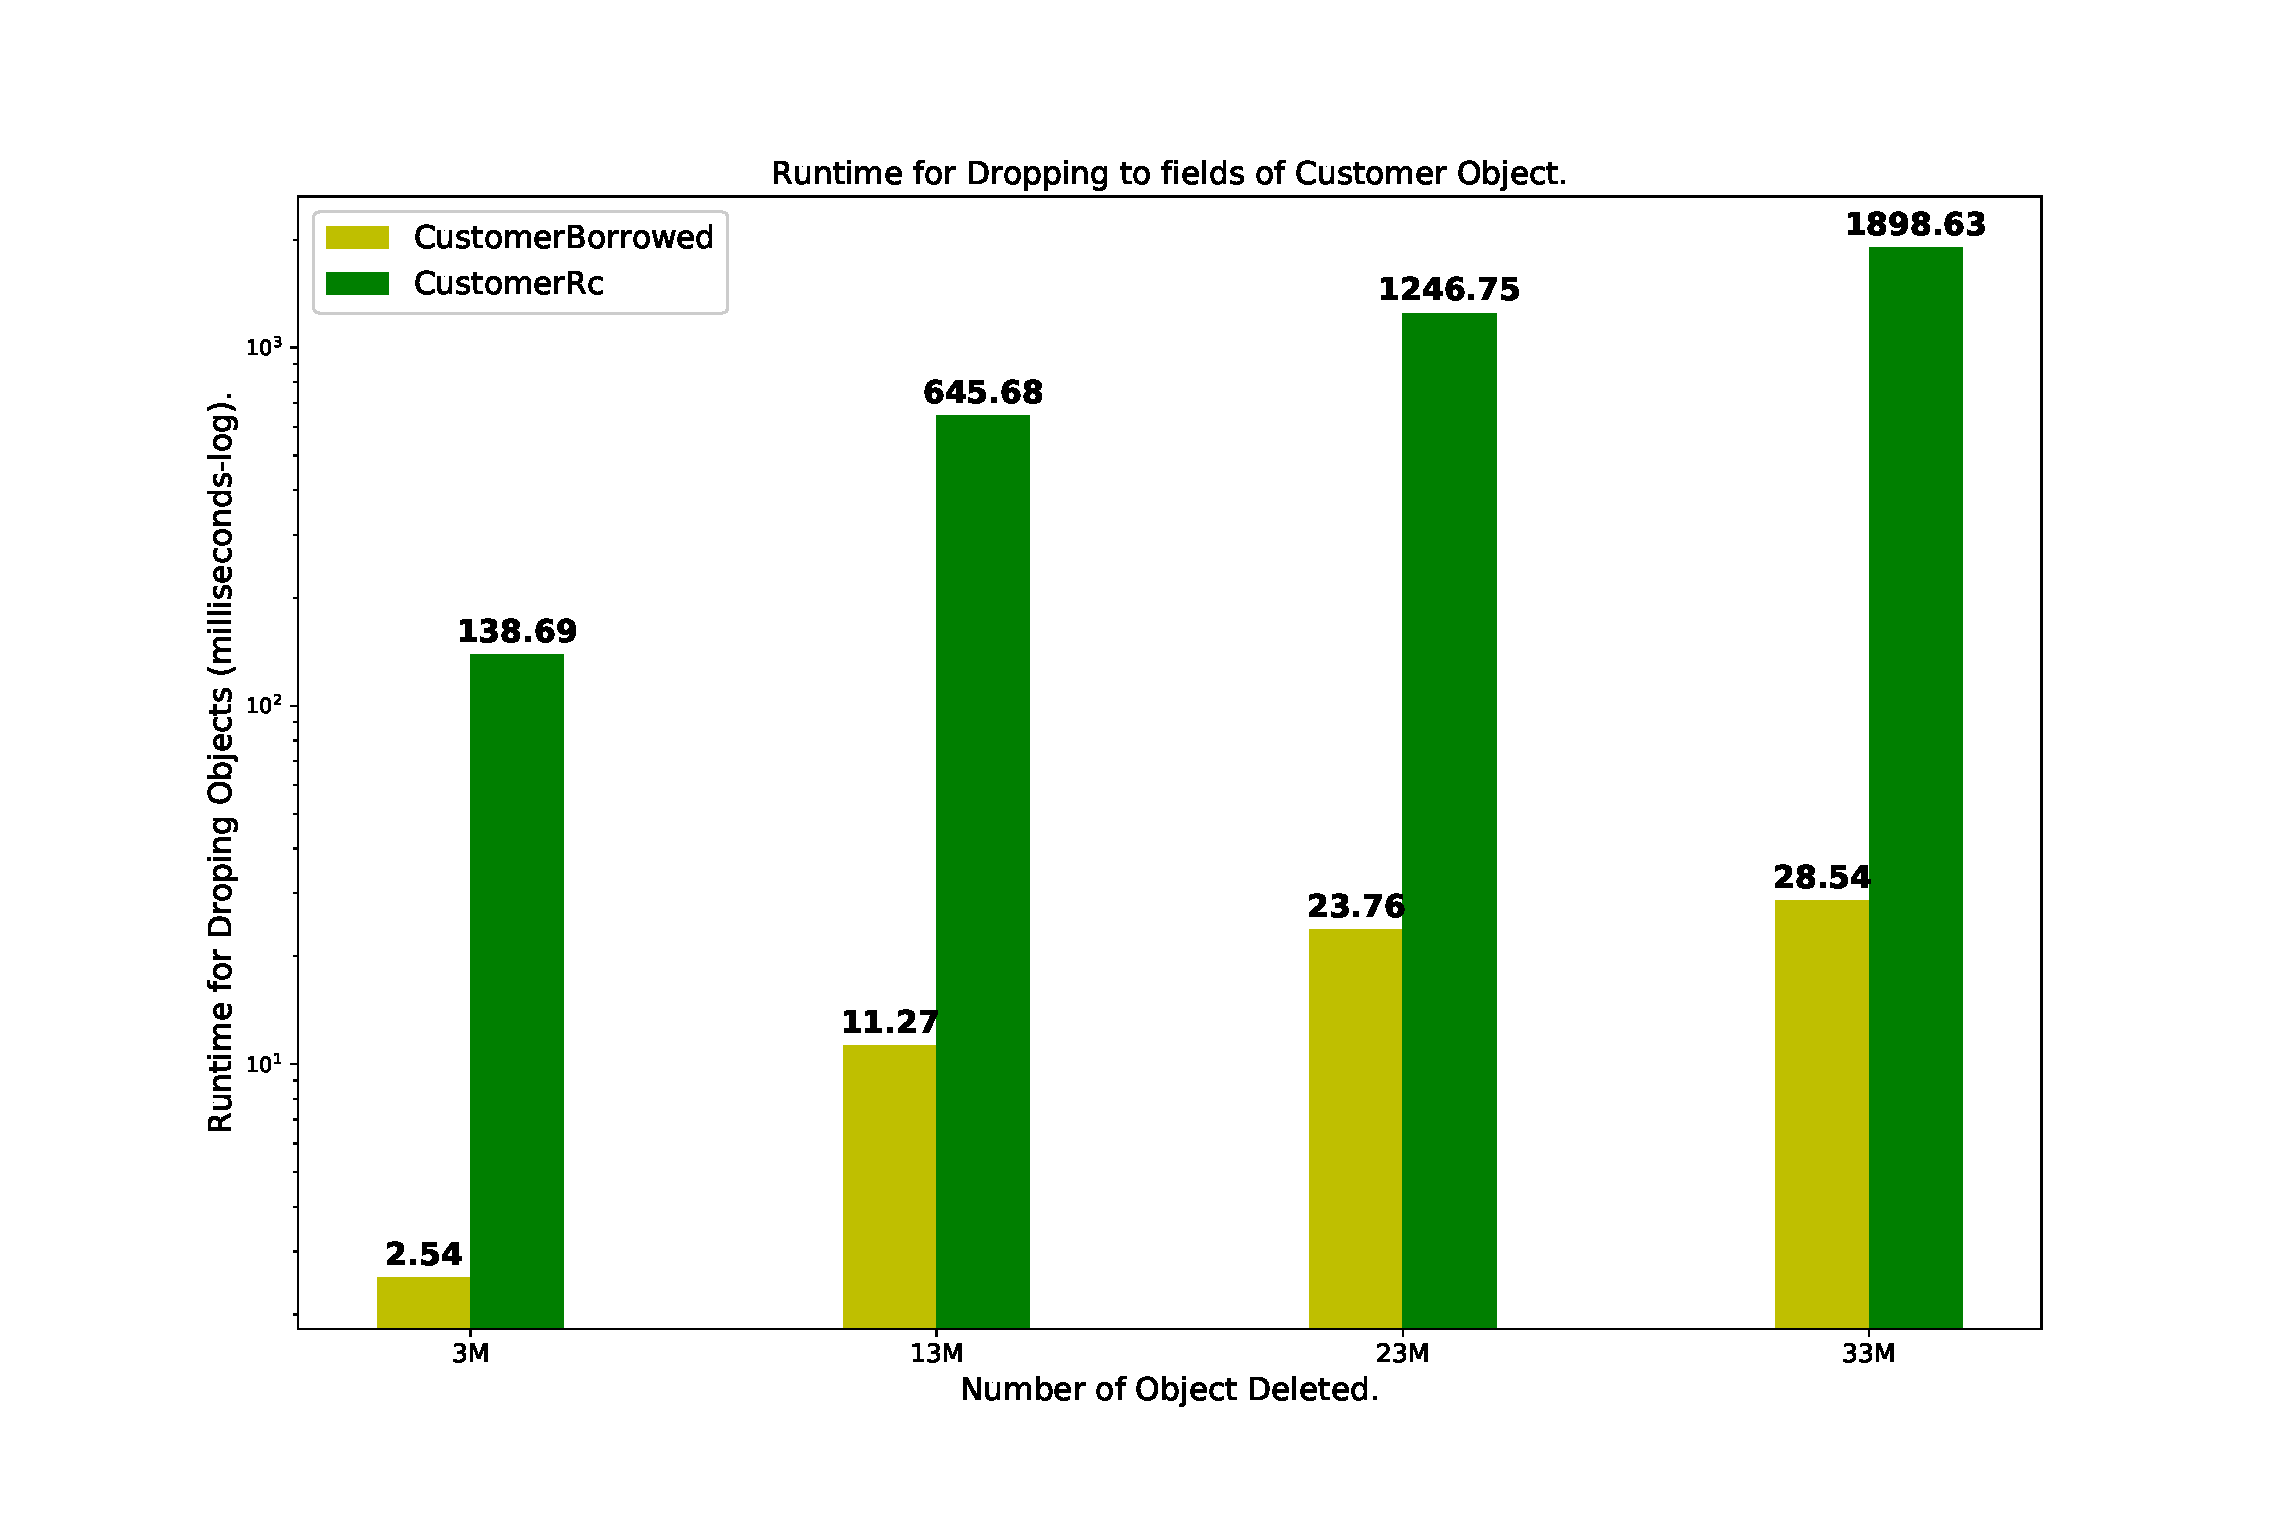
\includegraphics[width=15cm]{rust_droptime_borring_rc.eps}
    \caption{Runtime for dropping Customer Object}
    \label{fig:Sampling}
\end{figure}



\subsection{Discussion}
In this experiment, an assessment is conducted to verify whether there is difference between behavior of borrowing and reference counting. 
These two methods can be used in similar situation. Especially, when we want reference to an original variable and keep the original variable until all of references are dereferenced, 
we can have reference with both strategies, borrowing and reference counting. One advantage of using reference counting is that we do not have to pay attention to lifetime.
However, the assumption here is that use of reference counting might be computationally expensive than borrowing, because reference counting has to track the number of reference pointing to the value. 
Considered this assumption, we assess difference of time for dropping reference using borrowing and reference counting strategies. 